\documentclass[11pt, twocolumns]{article}

\usepackage{geometry}
\geometry{a4paper, left=2cm, top=2cm, right=2cm, bottom=2cm}

\usepackage[T1]{fontenc}
\usepackage[utf8]{inputenc}
\usepackage[spanish]{babel}
\usepackage{tikz}
\usepackage{url}
\usepackage{multicol}
\usepackage{float}
\usepackage{pgfplots}

\title{Comparativa de rendimiento PostgreSQL vs Crate}
\author{Tejero, Carlos Germán}

\begin{document}

\maketitle

\begin{abstract}
En la actualidad existe un explosión de almacenes de datos (principalmente bajo la denominación de NoSQL), los cuales implementan diferentes modelos de datos, a través de diferentes tecnologías y con características bastante diferentes que han dado por tierra el modelo ``One size fits all'' en el mundo de las bases de datos de datos. Dentro de este nuevo panorama, ha surgido Crate. Un gestor de bases de datos, orientado a la analítica de grandes volumenes de datos (principalmente de series de tiempo), con soporte para una arquitectura distribuida.
El siguiente trabajo presenta una comparativa de rendimiento entre PostgreSQL\cite{postgresql}, un gestor de base de datos relacional tradicional, y Crate\cite{crate}, un gestor de base de datos NoSQL con la particularidad de implementar un interfase SQL sobre un motor de búsquedas (search engine).
La comparativa ha sido realizada utilizando el \textit{benchmark} TPC-H\cite{tpc2018benchmark} y el software de pruebas Apache JMeter\cite{jmeter}.
\end{abstract}


\begin{multicols}{2}


\section{Introducción}
En la actualidad existe un explosión de almacenes de datos (principalmente bajo la denominación de NoSQL), los cuales implementan diferentes modelos de datos, a través de diferentes tecnologías y con características bastante diferentes que han dado por tierra el modelo ``One size fits all'' en el mundo de las bases de datos. Dentro de este nuevo panorama, ha surgido Crate. Un gestor de bases de datos, orientado a la analítica de grandes volumenes de datos (principalmente de series de tiempo), con soporte para una arquitectura distribuida.
\par
Una de las cacterísticas mas sobresalientes de Crate, es la combinación de un gestor de datos con soporte SQL, pero con un almacenamiento que hace uso de un motor de búsqueda, en este caso de Apache Lucene \cite{crate}.
\par
La pregunta que surge es ¿Cuanto mejor es el rendimiento para ejecutar cierto tipo de conultas, en comparación con un gestor de base de datos tradicional (relacional)?.
\par
Para intentar responder esta preguna en el presente trabajo, se ha realizado una comparativa de rendimiento, contrastando los resultados obtenidos de ejecutar el \textit{benchmark} (de ahora en más, punto de referencia) TPC-H en Crate y PostgreSQL, utilizando Apache JMeter.
\par
En las siguientes secciones se iran presentando una a una la herramientas elegidas para realizar la comparativa y los inconvenientes encontrados en el camino. Al final se encuentra el resultado de las pruebas realizadas, junto con la conclusión a la que se ha arribado, luego de relizado el trabajo.


\section{PostgreSQL}
Como figura en su documentación \cite{postgresql}, la historia de este gestor de bases de datos relacional, comienza en el año 1986, con el proyecto POSTGRES a cargo del profesor Michael Stonebraker. La primera demostración del mismo, fue presentada en la conferencia ACM-SIGMOD en el año 1988.
\par
En 1994 Andrew Yu and Jolly Chen agregarían un interprete del lenguaje SQL al proyecto, que sería renombrado como Postgre95, un sucesor de codigo abierto de POSTGRES.
\par
Ya en 1996, se modificó nuevamente su nombre a PostgreSQL para reflejar en forma más clara la relación entre el nombre original del proyecto POSTGRES y su compativilidad con SQL.
\par
En la actualidad PostgreSQL es un gestor de base de datos objeto-relacional destinado principalmente a OLTP y en menor medida a OLAP, de código abierto, muy apegado a los estandars SQL, que ofrece numerosas características avanzadas como:
\begin{itemize}
  \item Tipos de datos personalizados
	\item Herencia de tablas
  \item Transacciones anidadas
	\item MVCC
  \item Replicación física y lógica
	\item Espacios de tablas
	\item Particionamiento de tablas
	\item Y la posibilidad de todo tipo de extensiones
\end{itemize}
\par
Al momento de redactar este documento la última versión disponible es la 11.2, que se utilizó para la comparativa.


\section{Crate}
Crate es un gestor de base de datos de código abierto, para procesamiento en tiempo real y de datos producidos por máquinas. La primera versión fue lanzada por la empresa Crate.io en el año 2016.
\par
La característica más distintiva del producto, es que integra un gestor de base de datos SQL distribuido con un almacén de datos totalmente indexado y buscable, orientado a documentos.
\par
Utiliza el analizador de SQL de PrestoDB (FaceBook), Elasticsearch (Elasticsearch B.V.) and Lucene (Apache) para el transporte, busqueda y almacenamiento de los datos. Lo hace ideal para realizar rápidas búsquedas de texto y análisis de datos grandes volúmenes de datos de máquina.
\par
Al momento de escribir este documento, la ultima versión disponible del mismo es la 3.3.2 que se utilizó para la comparativa.


\section{TPC}
TPC es una corporación sin fines de lucro cuya misión es definir puntos de referencia (benchmarks) en el procesamiento de transacciones por gestores de  bases de datos, objetivos y verificables, capaces de ser difundidos.
\par
Los puntos de referencia producidos por TPC, permiten medir el desempeño del procesamiento de transacciones y del gestor de base de datos en términos de cuántas transacciones puede realizar un sistema y una base de datos determinados por unidad de tiempo, por ejemplo, transacciones por segundo o transacciones por minuto.
\par
El primer punto de referencia publicado fue TPC Benchmark A (TPC-A) en el año 1989, hoy en día obsoleto. En la actualidad TPC tiene numerosos puntos de referencia, de los que se destacan:
\begin{itemize}
  \item TCP-C
  \item TPC-E
  \item TPC-H
  \item TPC-DS
\end{itemize}
\par
Tanto TPC-C como TPC-E, son puntos de referencia orientados a OLTP. TPC-C es más viejo y simple, en cambio TPC-E es más moderno y complejo.
\par
TPC-H y TPC-DS son puntos de referencia orientados al soporte a la toma de desiciones. TPC-H consiste en un conjunto de consultas (22) ad-hoc que examina grandes volumenes de datos con un alto grado de complejidad. En cambio TCP-DS posee un complejo esquema estrella de data warehouse, con un gra número de consultas (100) complejas.
\par
Dado el alcance del presente trabajo, se decidió optar por realizar la comparativa utilizando el punto de referencia TPC-H, adaptado de forma de poder ejecutarse en los dos gestores de bases de datos elegidos (PostgreSQL y Crate).


\section{TPC-H}
La descripción de este punto de referencia, se encuantra en su especificacion \cite{tpc2018benchmark}:
TPC-H se compone de un conjunto de consultas de negocio (a las que se les ha dado un contexto realista) diseñado para ejercer las funcionalidades del sistema de bases de datos en una manera representativa de análisis de complejas aplicaciones de negocio.
\par
Auque una definicion más clara figura en \cite{scalzo2018database}:
TPC-H es una colección de 22 consultas SQL muy complejas, típicas para una base de datos de informes que soporta un sistema OLTP. Estas consultas tienen por objeto imitar las consultas de análisis de datos ad-hoc
de los usuarios finales, a través de herramientas de inteligencia de negocio con el fin de responder a preguntas críticas de negocios.
\par
El esquema de datos de TPC-H, es el típico de un sistema OLTP tradicional orientado a venta de productos, como se muestra en la Figura \ref{figura:tpch_esquema}. Cuenta con ocho (8) tablas:
\begin{enumerate}
  \item Region (continente)
  \item Nation (pais)
  \item Customer (cliente)
  \item Supplier (proveedor)
  \item Orders (pedido)
  \item LineItem (lineas de peido)
  \item Part (producto)
  \item PartSupp (producto-proveedor)
\end{enumerate}
\begin{figure}[H]
  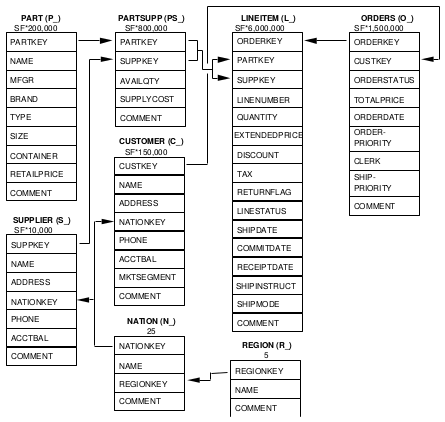
\includegraphics[scale=0.55]{tpch_esquema.png}
  \centering
  \caption{Esquema TPC-H (Extraido de \cite{tpc2018benchmark})}
  \label{figura:tpch_esquema}
\end{figure}
\par
Como ya fue menconado con antelación, cuenta con veintidos (22) consultas para ejecutar:
\begin{enumerate}
  \item Pricing Summary Report Query
  \item Minimum Cost Supplier Query
  \item Shipping Priority Query
  \item Order Priority Checking Query
  \item Local Supplier Volume Query
  \item Forecasting Revenue Change Query
  \item Volume Shipping Query
  \item National Market Share Query
  \item Product Type Profit Measure Query)
  \item Returned Item Reporting Query
  \item Important Stock Identification Query
  \item Shipping Modes and Order Priority Query
  \item Customer Distribution Query
  \item Promotion Effect Query
  \item Top Supplier Query
  \item Parts/Supplier Relationship Query
  \item Small-Quantity-Order Revenue Query
  \item Large Volume Customer Query
  \item Discounted Revenue Query
  \item Potential Part Promotion Query
  \item Suppliers Who Kept Orders Waiting Query
  \item Global Sales Opportunity Query
\end{enumerate}
\par
Además del esquema y las consultas, el punto de referencia cuenta con dos herramientas para generar el código SQL necesario para el gestor de base de datos elegido y los datos de carga. Estas herramientas son \textit{qgen}, el generado de SQL, y \textit{dbgen}, el generado de datos para poblar la base de datos.
\par
Ambas herramientas mencionadas, tienen soporte para los gestores de bases de datos: INFORMIX, DB2, Teradata, SQLSERVER, SYBASE, ORACLE y VECTORWISE, en los sistemas operativos ATT, DOS, HP, IBM, ICL, MVS, SGI, SUN, U2200, VMS, LINUX y WIN32. Esto supone un problema, dado que ninguno de los dos gestores elegidos para la comparativa estan soportados, por lo que se requiere realizar algunas adaptaciones al punto de referencia, para poder utilizarlo.


\section{Adaptaciones}
Como se emncionó anteriormente, TPC-H no tiene soporte para PostgreSQL y Crate. Para poder ser utilizado, se debieron realizar algunas adaptaciones y ajustes tanto al SQL/DDL para la creación del esquema, al SQL/DML de la consultas, como asi también a los datos de carga generados.
\par
Tanto para la generación de las consultas, como para la generación de los datos, se utilizó la opción de base de datos a ORACLE en el archivo \textit{Makefile} de TPC-H:
\begin{verbatim}
  DATABASE=ORACLE
\end{verbatim}
Esta opción fue considerada las más adecuada, dado que PostgreSQL tiene un alto grado de compatibilidad con ORACLE, y Crate busca versión tras versión alcanzar un mayor grado de compatibilidad con PostgreSQL.
Para la generación de las consultas, se utilizó la herramienta \textit{qgen}:
\begin{verbatim}
for q in `seq 1 22`; do
  DSS_QUERY=queries ./qgen $q > $q.sql
done
\end{verbatim}
Y para la generación de los datos, se utilizó la herramiento \textit{dbgen}:
\begin{verbatim}
./dbgen -s 1 -f  
\end{verbatim}

\subsection{Adaptaciones para PostgreSQL}
Para poder utilizar TPC-H con PostgreSQL no es necesario realizar grandes cambios. Sólo fueron requeridas dos pequeñas modificaciones a las consultas y a los datos generados.

\subsubsection{Adaptaciones a las consultas}
Las consultas generedas para ORACLE, utilizan un mecanimos no estándar para limitar la cantidad de filas del resultado. Por ejemplo en la consulta \textit{1}:
\begin{verbatim}
WHERE rownum <= -1;
\end{verbatim}
Este podría haberse reemplazado por un mecanismo más estandar (FETCH FIRST..), sin embargo se decidió utilizar uno propio de PostgreSQL, ya que tambien es soportado por Crate. De esta forma cada consulta fue modificada, como por ejemplo la consulta \textit{1}:
\begin{verbatim}
LIMIT 1;
\end{verbatim}

\subsubsection{Adaptaciones a datos generados}
Los datos generados utilizando un formato similar a \textit{CSV}, utilizando el caracter \textit{|} como separador de registro, con extension \textit{.tbl}. Estos archivos pueden ser facilmente cargados utilizando la sentencia \textit{COPY} de PostgreSQL, a no ser porque los mismos incluyen un caracter \textit{|} despues del ultimo registro. Para poder cargarlos se debió remover este caracter demás:
\begin{verbatim}
sed -i 's/|$//g' $i *.tbl
\end{verbatim}

\subsection{Adaptaciones para Crate}
Dado que Crate es un gestor bastante reciente, posee aun numerosas limitaciones en comparación con gestores más antiguos y maduros. Esto hizo necesario relizar numerosas adaptaciones, a fin de poder utilizar TPC-H.

\subsubsection{Adaptaciones al esquema}
Para la creación del esquema de la base de datos de TPC-H, se encontraron varias limitacione en cuanto a los tipos de datos soportados por Crate \cite{crate}. Los datos no soportdos utilizados por TPC-H fueron:
\begin{itemize}
  \item DATE
  \item DECIMAL(15,2)
  \item CHAR
\end{itemize}
Para salvar esta limitación se decidió reemplazar en la definición de la estructura cada tipo de datos no soportado, por un tipo de datos soportado de similares características. Los reemplazos realizados fueron:
\begin{itemize}
  \item DATE por TIMESTAMP
  \item DECIMAL(15,2) por DOUBLE
  \item CHAR por VARCHAR
\end{itemize}
Para hacer más justa la comparativa de rendimiento, y teniendo en cuenta que al modificar los tipos de datos, también se introducen diferencias en el procesamiento de los mismos, estos cambios también fueron introducidos en la definición del esquema para PostgreSQL.
  
\subsubsection{Adaptaciones a las consultas}
Para las consultas, nuevamente se encontraron numerosas limitaciones. Las que pudieron se salvadas con pequeñas modificaciones, se hicieron. Pero las que hicieron imposible la ejecución de alguna consulta, hicieron necesaria descartar la consulta no soportada.
\par
Una limitación encontrada, fué el pobre soporte para expresiones dentro de las consultas. Por ejemplo, en la clausula \textit{WHERE} de la consulta \textit{1}:
\begin{verbatim}
WHERE l_shipdate >= '1993-09-01'
  AND l_shipdate  < '1993-09-01' 
                  + INTERVAL '3' MONTH  
\end{verbatim}
Fue necesario reescribirla, eliminando la expresión y tansformandola en una constante:
\begin{verbatim}
WHERE l_shipdate >= '1993-09-01'
  AND l_shipdate  < '1993-12-01'  
  
\end{verbatim}
De igual forma se procedió con todas las consultas que contenian expresiones no soportadas.
\par
Otra limitación encontrada, fue que Crate solo posee soporte para subconsultas no correlacionadas \cite{crate}. Esto no permite ejecutar ciertas de las consultas incluidas en TPC-H, dado que las mismas contienen este tipo de subconsultas:
\begin{itemize}
  \item [2.] Minimum Cost Supplier Query
  \item [4.] Order Priority Checking Query
  \item [17.] Small-Quantity-Order Revenue Query
  \item [20.] Potential Part Promotion Query
  \item [21.] Suppliers Who Kept Orders Waiting Query
  \item [22.] Global Sales Opportunity Query
\end{itemize}
Asi mismo, otra limitación encontrada, es la carencia de un planificador sofisticado \cite{crate}, como el presente en la mayoría de los gestores de bases de datos maduros. Sumado a esto, se encuentra el hecho de que para ejecutar reuniones, solo posee soporte para el algoritmo \textit{hash join} (A menos que se fuerce un \textit{nested loop join}). Esto hace que consultas que incluyan varias tablas en la clausula \textit{FROM}, sean extremadamente lentas y requieran enormes cantidades de memoria. Como eurística, se procedió a no utilizar consultas que incluyan mas de tres (3) tablas en la cláusula \textit{FROM}. De esta forma se vieron descartadas las consultas:
\begin{itemize}
  \item [5.] Local Supplier Volume Query
  \item [7.] Volume Shipping Query
  \item [8.] National Market Share Query
  \item [9.] Product Type Profit Measure Query
  \item [10.] Returned Item Reporting Query
\end{itemize}
La misma carencia de planificador, hizo que algunas consultas fueran imposibles de considerar. Incluso no se obtuvo resultado de las mismas, a pesar de esperar horas por su terminación. Por lo que se dejó fuera también las consultas:
\begin{itemize}
  \item [13.] Customer Distribution Query
  \item [19.] Discounted Revenue Query
\end{itemize}
Dadas todas las limitaciones mencionadas, se decidió solamente realizar la comparativa utilizando las consultas:
\begin{itemize}
  \item [1.] Pricing Summary Report Query
  \item [3.] Shipping Priority Query
  \item [6.] Forecasting Revenue Change Query
  \item [11.] Important Stock Identification Query
  \item [12.] Shipping Modes and Order Priority Query
  \item [14.] Promotion Effect Query
  \item [15.] Top Supplier Query
  \item [16.] Parts/Supplier Relationship Query
  \item [18.] Large Volume Customer Query
\end{itemize}

\subsubsection{Adaptaciones a datos generados}
Si bien Crate posee la sentencia \textit{COPY}, similar a PostgreSQL, esta posee muchas menos opciones de configuración. Esta sentencia solo permite cargar archivo \textit{CSV}, utilizando el caracter \textit{,} como separado de registro y el caracter \textit{"} para delimitar cadenas de caracteres.
\par
Para saltar estas limitaciones, se procedió a realizar el volcado de los datos desde PostgreSQL directamente en el formato esperado. Esto genera realizar un paso demás, ya que se deben cargar los datos primero en PostgreSQL para luego volcarlos nuevamente a archivos que puedan ser cargados por Crate. Pero no produce ningun tipo de interferencia en la realización de las pruebas. 


\section{JMeter}
JMeter es una herramienta de código abierto mantenido por la Fundación apache para realizar pruebas de rendimiento de nivel industrial. Es un proyecto muy maduro, continuamente actualizado y revizado desde su creación en 2001.
\par
Como indica su página \cite{jmeter}, puede ser utilizado para probar el rendimiento tanto en recursos estáticos como dinámicos. Es capaz de simular carga a un servidor o grupo de servidores, para probar o para analizar el rendimiento general bajo diferentes tipos de carga.
\par
Las principales características de Apache JMeter incluyen:
\begin{itemize}
  \item Capacidad probar el rendimiento de:
  \begin{itemize}
    \item Aplicaciones Web (HTTP, HTTPS, etc)
    \item Servicios Web SOAP / REST
    \item FTP
    \item Base de datos a través de JDBC
    \item LDAP
    \item Middleware orientado a mensajes (JMS)
    \item Correo - SMTP(S), POP3(S) e IMAP(S)
  \end{itemize}
  \item IDE de prueba completo que permite la creación y la depuración del plan de prueba.
  \item Modo de línea de comandos ejecutar las pruebas.
  \item Completos informes en diferentes formatos de salida.
  \item Portabilidad completa (100\% Java).
  \item Soporte para muestreo simultáneo a través de múltiples subprocesos.
  \item La posibilidad de realizar extensiones.
\end{itemize}
Al momento de escribir este documento, la ultima versión disponible de JMeter es la 5.1.1 que se utilizó para la comparativa.


\section{Comparativa de rendimiento}
Para ejecutar la comparativa de rendimiento, se utilizó una máquina virtual a través de Vagrant con las siguientes características:
\begin{enumerate}
  \item CPUS: 3
  \item RAM: 5120MB
  \item Disco: 40GB
  \item Sistemas operativo: centos/7
\end{enumerate}
Además se realizaron cuatro planes de prueba \cite{matam2017performance}:
\begin{enumerate}
  \item Un plan de prueba para la carga de datos en Postgresql (CrateLoad.jmx).
  \item Un plan de prueba para la carga de datos en Crate (CrateQuery.jmx).
  \item Un plan de prueba de las consultas para PostgreSQL (PostgreSQLLoad.jmx).
  \item Un plan de prueba de las consultas para Crate (PostgreSQLQuery.jmx).
\end{enumerate}

\subsubsection{Plan de prueba para carga}
El plan de prueba de la carga de datos de ambos gestores, se realizaron incluyendo los siguientes elementos (como se muestra en la Figura \ref{figura:plan_carga_pg}):
\begin{itemize}
  \item Grupo de hilos (Thread Group): Que modela la ejecución por parte de un único hilo, la ejecución de las sentencias de carga, una a una, de forma secuencial, una única vez.
  \item Configuración de la conexión JDBC (JDBC Connecton Configuration): Que contiene los datos para realiza la conexión al gestor. 
  \item Peticiones JDBC (JDBC Request): Se incluye uno por cada tabla a cargar (8).
  \item Reporte de resultados (Summary report): Se incluye un reporte para obtener los resultados de la ejecución de la prueba.
\end{itemize}
Cada una de las peticiones JDBC para la arga de datos, utiliza la sentencia \textit{COPY} (con las variantes de cada gestor). Por ejemplo para la carga de la tabla de paises (nation): 
\begin{verbatim}
COPY nation FROM '/tmp/nation.csv';
\end{verbatim}
Para realizar la comparativa de rendimiento de carga, se tomará del reporte de resultado el tiempo medido en milisegundos que demora cada gestor en realizar la carga de los datos de cada una de las tablas y el tiempo total.
\begin{figure}[H]
  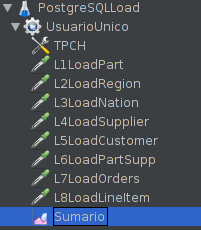
\includegraphics[scale=0.7]{plan_carga_pg.png}
  \centering
  \caption{Plan de prueba para carga de datos}
  \label{figura:plan_carga_pg}
\end{figure}

\subsubsection{Plan de prueba para consultas}
El plan de prueba para la ejecución de las consultas en ambos gestores, se realizaron incluyendo los siguientes elementos (como se muestra en la Figura \ref{figura:plan_consultas_pg}):
\begin{itemize}
  \item Grupo de hilos (Thread Group): Que modela la ejecución por parte de un único hilo, la ejecución de las consultas, una a una, de forma secuencial, diez (10) veces.
  \item Configuración de la conexión JDBC (JDBC Connecton Configuration): Que contiene los datos para realiza la conexión al gestor. 
  \item Peticiones JDBC (JDBC Request): Se incluye uno por cada consulta a ejecutar.
  \item Reporte de resultados (Summary report): Se incluye un reporte para obtener los resultados de la ejecución de la prueba.
\end{itemize}
Cada una de las peticiones JDBC para las consultas, contiene la consula del punto de referencia TCP-H a ejecutar.
\par
Para realizar la comparativa de rendimiento de las consultas, se tomará del reporte de resultado el tiempo medio medido en milisegundos que demora cada gestor en realizar la ejecución de cada una de las consultas y el tiempo total.
\begin{figure}[H]
  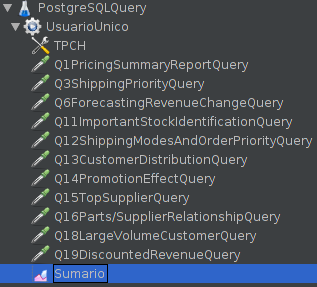
\includegraphics[scale=0.7]{plan_consultas_pg.png}
  \centering
  \caption{Plan de prueba para consultas}
  \label{figura:plan_consultas_pg}
\end{figure}


\section{Resultados}
A continuación, se encuentran los resultados obtenidos. Se presentan por separado los resultados del plan de pruebas de carga de datos, y en forma detallada los resutados para cada una de las consultas ejecutadas.

\subsection{Carga de datos}
Los resultados obtenidos se muestran en la Figura \ref{gráfico:gr_resultado_carga}. En esta prueba se cometió una gran error, ya que Crate indexa de forma predeterminada todos los datos almacenados en cada una de las tablas, por lo que al cargar los datos estos son indexados. En la carga de datos en PostgreSQL, se separó la carga de los datos en las tablas sin restricciones ni índices definidos, para luego definir las restricciones y los índices ni bien se termine la carga de los mismos. Esto es una práctica habitual en el mundo de las bases de datos relacionales, para mejorar los tiempos de carga. Pero al no poder ejecutar sentencias \textit{SQL/DDL} a través de la herramienta JMeter, no se pudo medir el tiempo demorado en la ejecución de las mismas.
\par
Como se ve en la Figura \ref{gráfico:gr_resultado_carga}, las diferencias de rendimiento son bastante marcadas, principalmente producto del error cometido. Esto produjo que los resultados de la prueba, no se tengan en cuenta para las conclusiones, ya que no se contó con tiempo para enmendar el error.

\begin{figure}[H]
\begin{tikzpicture}
	\begin{axis}[
		legend style={at={(0.5, -0.2)}, anchor=north, legend columns=-1},
		ylabel={Milisegundos},
		xlabel={Filas (en millones)}
	]
  \addplot coordinates {(30, 471679) (24, 359295) (18, 270309) (12, 182024) (6,  90047)};
  \addplot coordinates {(30,5484797) (24,4766563) (18,3557494) (12,2241889) (6,1060600)};
	\legend{PostgreSQL,Crate}
	\end{axis}
\end{tikzpicture}
    \caption{Comparación de rendimiento de carga}
	\label{gráfico:gr_resultado_carga}
\end{figure}


\subsection{Q1 Pricing Summary Report Query}
La consulta Q1, combina agrupamiento y agregación sobre la tabla \textit{lineitem}, la que contiene más filas en la base de datos. En este caso, a partir de los resultados, se ve como Crate tiene un mejor rendimiento por sobre PostgreSQL, en consultas sobre pocas tablas con gran cardinalidad.
Los resultados obtenidos se muestran en la Figura \ref{gráfico:gr_resultado_q1}.

\begin{figure}[H]
\begin{tikzpicture}
	\begin{axis}[
		legend style={at={(0.5, -0.2)}, anchor=north, legend columns=-1},
		ylabel={Milisegundos},
		xlabel={Filas (en millones)}
	]
	\addplot coordinates {(30,105310) (24,61355) (18,23531) (12, 8731) (6,3912)};
  \addplot coordinates {(30, 31574) (24,24438) (18,21696) (12,15504) (6,9887)};
	\legend{PostgreSQL,Crate}
	\end{axis}
\end{tikzpicture}
    \caption{Comparación de rendimiento Q1}
	\label{gráfico:gr_resultado_q1}
\end{figure}

\subsection{Q3 Shipping Priority Query}
La consulta Q3, realiza una reunión entre tres (3) tablas, combina filtrado, agrupamiento y agregación. En este caso, se ve la superioridad de rendimiento de PostgreSQL por sobre Crate, y la carencia de un planificador por parte de este último.
\par
Los resultados obtenidos se muestran en la Figura \ref{gráfico:gr_resultado_q3}.

\begin{figure}[H]
\begin{tikzpicture}
	\begin{axis}[
		legend style={at={(0.5, -0.2)}, anchor=north, legend columns=-1},
		ylabel={Milisegundos},
		xlabel={Filas (en millones)}
	]
	\addplot coordinates {(30, 94364) (24, 53069) (18, 15089) (12, 3139) (6,1225)};
  \addplot coordinates {(30,256772) (24,182794) (18,107531) (12,14743) (6,7472)};
	\legend{PostgreSQL,Crate}
	\end{axis}
\end{tikzpicture}
    \caption{Comparación de rendimiento Q3}
	\label{gráfico:gr_resultado_q3}
\end{figure}


\subsection{Q6 Forecasting Revenue Change Query}
La consulta Q6, realiza una agregación sobre una sola tabla, y el filtrado de la misma. Nuevamente como en la consulta Q1, se ve nuevamente la mejora de rendimiento de Crate.
\par
Los resultados obtenidos se muestran en la Figura \ref{gráfico:gr_resultado_q6}.

\begin{figure}[H]
\begin{tikzpicture}
	\begin{axis}[
		legend style={at={(0.5, -0.2)}, anchor=north, legend columns=-1},
		ylabel={Milisegundos},
		xlabel={Filas (en millones)}
	]
	\addplot coordinates {(30,63710) (24, 4506) (18,3244) (12,2663) (6,880)};
	\addplot coordinates {(30, 13646) (24,9657) (18,9204) (12,2869) (6,982)};
	\legend{PostgreSQL,Crate}
	\end{axis}
\end{tikzpicture}
    \caption{Comparación de rendimiento Q6}
	\label{gráfico:gr_resultado_q6}
\end{figure}


\subsection{Q11 Important Stock Identification Query}
La consulta Q11, realiza la reunión entres tres (3) tablas, agrupamiento, agregación, filtrado, combinado con una subconsulta. En este caso se ve nuevamente la mejora de rendimiento de PostgreSQL, aunque la misma no es muy significativa.
\par
Los resultados obtenidos se muestran en la Figura \ref{gráfico:gr_resultado_q11}.

\begin{figure}[H]
\begin{tikzpicture}
	\begin{axis}[
		legend style={at={(0.5, -0.2)}, anchor=north, legend columns=-1},
		ylabel={Milisegundos},
		xlabel={Filas (en millones)}
	]
  \addplot coordinates {(30,22587) (24,20633) (18,16669) (12,13195) (6, 605)};
	\addplot coordinates {(30,27485) (24,24236) (18,17769) (12,12601) (6,5740)};
	\legend{PostgreSQL,Crate}
	\end{axis}
\end{tikzpicture}
    \caption{Comparación de rendimiento Q11}
	\label{gráfico:gr_resultado_q11}
\end{figure}


\subsection{Q12 Shipping Modes and Order Priority Query}
La consulta Q12, realiza la reunión de dos (2) tablas, agrupamiento, agregación y filtrado. Nuevamente se ve una mejora de rendimiento de Crate por PostgreSQL.
\par
Los resultados obtenidos se muestran en la Figura \ref{gráfico:gr_resultado_q12}.

\begin{figure}[H]
\begin{tikzpicture}
	\begin{axis}[
		legend style={at={(0.5, -0.2)}, anchor=north, legend columns=-1},
		ylabel={Milisegundos},
		xlabel={Filas (en millones)}
	]
	\addplot coordinates {(30,63196) (24,30848) (18, 4331) (12, 3506) (6,1753)};
	\addplot coordinates {(30,20223) (24,19109) (18,17696) (12,12506) (6,5235)};
	\legend{PostgreSQL,Crate}
	\end{axis}
\end{tikzpicture}
    \caption{Comparación de rendimiento Q12}
	\label{gráfico:gr_resultado_q12}
\end{figure}


\subsection{Q14 Promotion Effect Query}
La consulta Q14, realiza la reunión de dos (2) tablas, filtrado y agregación. Nuevamente se puede apreciar como al aumentar el número de filas en las tablas involucradas en consultas con pocas tablas, Crate comienza a tener un mejor rendimiento.
\par
Los resultados obtenidos se muestran en la Figura \ref{gráfico:gr_resultado_q14}.

\begin{figure}[H]
\begin{tikzpicture}
	\begin{axis}[
		legend style={at={(0.5, -0.2)}, anchor=north, legend columns=-1},
		ylabel={Milisegundos},
		xlabel={Filas (en millones)}
	]
	\addplot coordinates {(30,35200) (24,5922) (18,2808) (12,1162) (6, 493)};
	\addplot coordinates {(30, 9329) (24,7816) (18,4375) (12,2749) (6,1290)};
	\legend{PostgreSQL,Crate}
	\end{axis}
\end{tikzpicture}
    \caption{Comparación de rendimiento Q14}
	\label{gráfico:gr_resultado_q14}
\end{figure}


\subsection{Q15 Top Supplier Query}
La consulta Q15, reliza la reunion de una (1) tabla con una (1) vista de agrupamiento y agregación. Nuevamente se ve un mejora rendimiento de Create por PostgreSQL.
Los resultados obtenidos se muestran en la Figura \ref{gráfico:gr_resultado_q15}.

\begin{figure}[H]
\begin{tikzpicture}
	\begin{axis}[
		legend style={at={(0.5, -0.2)}, anchor=north, legend columns=-1},
		ylabel={Milisegundos},
		xlabel={Filas (en millones)}
	]
	\addplot coordinates {(30,31947) (24,8047) (18,3957) (12,3781) (6,1589)};
	\addplot coordinates {(30, 6576) (24,4537) (18,3372) (12,2394) (6, 851)};
	\legend{PostgreSQL,Crate}
	\end{axis}
\end{tikzpicture}
    \caption{Comparación de rendimiento Q15}
	\label{gráfico:gr_resultado_q15}
\end{figure}


\subsection{Q16 Parts/Supplier Relationship Query}
La consulta Q16, realiza una reunión entre dos (2) tablas, agrupamiento, agregación y filtrado haciendo uso de una subconsulta. En este caso no se ve una diferencia significativa de rendimiento de uno por sobre el otro.
\par
Los resultados obtenidos se muestran en la Figura \ref{gráfico:gr_resultado_q16}.

\begin{figure}[H]
\begin{tikzpicture}
	\begin{axis}[
		legend style={at={(0.5, -0.2)}, anchor=north, legend columns=-1},
		ylabel={Milisegundos},
		xlabel={Filas (en millones)}
	]
	\addplot coordinates {(30,16213) (24,12719) (18,2756) (12,1882) (6, 969)};
	\addplot coordinates {(30,14006) (24,13776) (18,7754) (12,5437) (6,2565)};
	\legend{PostgreSQL,Crate}
	\end{axis}
\end{tikzpicture}
    \caption{Comparación de rendimiento Q16}
	\label{gráfico:gr_resultado_q16}
\end{figure}


\subsection{Q18 Large Volume Customer Query}
La consutla Q18, realiza la reunión de tres (3) tablas, agrupamiento, agregación y filtrado con una subconsulta. Nuevamente no se ve una diferencia de rendimiento significativa de uno por sobre el otro.
\par
Los resultados obtenidos se muestran en la Figura \ref{gráfico:gr_resultado_q18}.

\begin{figure}[H]
\begin{tikzpicture}
	\begin{axis}[
		legend style={at={(0.5, -0.2)}, anchor=north, legend columns=-1},
		ylabel={Milisegundos},
		xlabel={Filas (en millones)}
	]
	\addplot coordinates {(30,114310) (24, 24413) (18,11100) (12, 5457) (6,2374)};
	\addplot coordinates {(30,118856) (24,100263) (18,64799) (12,16498) (6,6721)};
	\legend{PostgreSQL,Crate}
	\end{axis}
\end{tikzpicture}
    \caption{Comparación de rendimiento Q18}
	\label{gráfico:gr_resultado_q18}
\end{figure}


\section{Conclusiones}
A pesar de las limitaciones encontradas en Crate, los resultados obtenidos en las pruebas de rendimiento dejan ver que su rendimiento ha sido bastante similar en la mayoría de los casos, a los obtenidos por PostgreSQL salvo en los casos en que las consultas se realizaran sobre una o dos tablas con gran número de filas. Esto, a pesar de haber utilizado el punto de referencia TPC-H, que posee una estructura de base de datos estilo OLTP. Los resultados permiten suponer que en pruebas de rendimiento sobre bases de datos con modelos más adecuados para Crate, la diferencia de rendimiento comience a ser más significativa.
\par
Es de destacar, que en las pruebas realizadas no se han hecho uso de características destacadas de Crate como su posibilidad de distribución o \textit{sharding}. Lo que mejoraría significativamente el rendimiento para la ejecución las pruebas.


\bibliographystyle{acm}
\bibliography{bibliografia}


\end{multicols}

\end{document}
